%% -*- latex -*-
%%%%%%%%%%%%%%%%%%%%%%%%%%%%%%%%%%%%%%%%%%%%%%%%%%%%%%%%%%%%%%%%
%%%%
%%%% This TeX file is part of the course
%%%% Introduction to Scientific Programming in C++/Fortran2003
%%%% copyright 2021-2023 Victor Eijkhout eijkhout@tacc.utexas.edu
%%%%
%%%% zerofind.tex : exercises about zero finding
%%%%
%%%%%%%%%%%%%%%%%%%%%%%%%%%%%%%%%%%%%%%%%%%%%%%%%%%%%%%%%%%%%%%%

\Level 0 {Root finding by bisection}
\label{sec:root-bisection}

\begin{figure}[ht]
  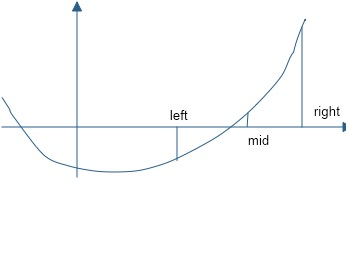
\includegraphics[scale=.6]{zerofind}
  \caption{Root finding by interval bisection}
  \label{fig:zerofind}
\end{figure}

For many functions~$f$, finding their zeros, that is, the values~$x$
for which~$f(x)=0$, can not be done analytically. You then have to
resort to numerical \indexterm{root finding} schemes.
In this project you will develop gradually more complicated
implementations of a simple scheme:
root finding by \indexterm{bisection}.

In this scheme, you start with two points where the function has opposite signs,
and move either the left or right point to the mid point,
depending on what sign the function has there.
See figure~\ref{fig:zerofind}.

In section~\ref{sec:newton} we will then look at Newton's method.

Here we will not be interested in mathematical differences between the methods,
though these are important:
we will use these methods to exercise some programming techniques.

\Level 1 {Simple implementation}
\label{sec:rootfindarray}

\prerequisite{ch:function}
\prerequisite{ch:array}

Let's develop a first implementation step by step.
To ensure correctness of our code we will use a \acf{TDD} approach:
for each bit of functionality we write a test
to ensure its correctness before we integrate it in the larger code.
(For more about \ac{TDD}, and in particular the Catch2 framework,
see section~\ISPref{sec:tdd}.)

\Level 1 {Polynomials}

First of all, we need to have a way to represent polynomials.
For a polynomial of degree~$d$ we need $d+1$ coefficients:
\begin{equation}
  f(x) = c_0 x^d + \cdots + c_{d-1} x^1 + c_d
  \label{eq:poly-coeff}
\end{equation}
We implement this by storing the coefficients in a
\lstinline+vector<double>+.
We make the following arbitrary decisions
\begin{enumerate}
\item let the first element
  of this vector be the coefficient of the highest power, and
\item 
  for the coefficients to properly define a polynomial,
  this leading coefficient has to be nonzero.
\end{enumerate}
Let's start by having a fixed test polynomial,
provided by a function \lstinline+set_coefficients+.
For this function to provide a proper polynomial,
it has to satisfy the following test:
%
\verbatimsnippet{rootproperpoly}

\begin{exercise}
  \label{ex:bisect-coeff}
  Write a routine \lstinline+set_coefficients+ that constructs
  a vector of coefficients:
  \verbatimsnippet{rootsetcoeffcall}
  and make it satisfy the above conditions.
  
  At first write a hard-coded set of coefficients,
  then try reading them from the command line.
\end{exercise}

Above we postulated two conditions that an array of numbers should satisfy
to qualify as the coefficients of a polynomial.
Your code will probably be testing for this,
so let's introduce a boolean function
\lstinline+is_proper_polynomial+:
\begin{itemize}
\item This function returns \lstinline{true} if the array of numbers satisfies
  the two conditions;
\item it returns \lstinline{false} if either condition is not satisfied.
\end{itemize}

In order to test your function \lstinline+is_proper_polynomial+ you should check that
\begin{itemize}
\item
  it recognizes correct polynomials, and
\item it fails for improper coefficients that do not properly define a polynomial.
\end{itemize}

\begin{exercise}
  \label{ex:proper-poly}
  Write a function \lstinline+is_proper_polynomial+ as described,
  and write unit tests for it, both passing and failing:
\begin{lstlisting}
  vector<double> good = /* proper coefficients */ ;
  REQUIRE( is_proper_polynomial(good) );
  vector<double> notso = /* improper coefficients */ ;
  REQUIRE( not is_proper_polynomial(good) );
\end{lstlisting}
\end{exercise}

Next we need polynomial evaluation.
We will build a function \lstinline{evaluate_at} with the
following definition:
\verbatimsnippet{evaluateatproto}

You can interpret the array of coefficients in
(at least) two ways, but with equation~\eqref{eq:poly-coeff}
we proscribed one particular interpretation.

So we need a  test that the coefficients are
indeed interpreted with the leading coefficient first,
and not with the leading coefficient last.
For instance:
%
\verbatimsnippet{rootcatcheval}
%
(where we have left out the \lstinline+TEST_CASE+ header.)

Now we write the function that passes these tests:

\begin{exercise}
  \label{ex:bisect-eval}
  Write a function \lstinline+evaluate_at+ which computes
  \[ y \leftarrow f(x) . \]
  and confirm that it passes the above tests.
\begin{lstlisting}
double evaluate_at( polynomial coefficients,double x);
\end{lstlisting}
  For bonus points, look up \indexterm{Horner's rule}
  and implement it.
\end{exercise}

With the polynomial function implemented,
we can start working towards the algorithm.

\Level 1 {Left/right search points}

\begin{figure}[ht]
  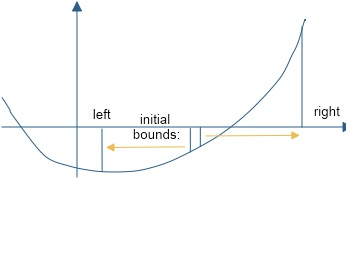
\includegraphics[scale=.6]{zero-outer}
  \caption{Setting the initial search points}
  \label{fig:zero-outer}
\end{figure}

Suppose $x_-,x_+$ are such that 
\[ x_-<x_+,\quad\hbox{and}\quad f(x_-)\cdot f(x_+)<0,\]
that is, the function values in the left and right point are of opposite sign.
Then there is a zero in the interval~$(x_-,x_+)$;
see figure~\ref{fig:zerofind}.

But how to find these outer bounds on the search?

If the polynomial is of odd degree you can find $x_-,x_+$
by going far enough to the left and right
from any two starting points.
For even degree there is no such simple algorithm
(indeed, there may not be a zero)
so we abandon the attempt.

We start by writing a function \lstinline+is_odd+ that tests
whether the polynomial is of odd degree.

\begin{exercise}
  \label{ex:bisect-odd}
  Make the following code work:
  \verbatimsnippet{rootoddcall}
\end{exercise}

You could test the above as:
\verbatimsnippet{rootcatchodd}

Now we can find $x_-,x_+$: start with some interval
and move the end points out until the function values have opposite sign.

\begin{exercise}
  \label{ex:bisect-outer}
  Write a function \lstinline+find_initial_bounds+ which computes $x_-,x_+$
  such that
  \[ f(x_-)<0<f(x_+) \quad\hbox{or}\quad f(x_+)<0<f(x_-) \]
  How can you compute this test more compactly?\\
  What is a good prototype for the function?\\
  How do move the points far enough out to satisfy this condition?
\end{exercise}

Since finding a left and right point with a zero in between is not always
possible for polynomials of even degree, we completely reject this case.
In the following test we throw an exception
(see section~\ISPref{sec:exception}, in particularly~\ISPref{sec:except-throw})
for polynomials of even degree:
\verbatimsnippet{rootcatchouter}
Make sure your code passes these tests.
What test do you need to add
for the function values?

\Level 1 {Root finding}

The root finding process globally looks as follows:
\begin{itemize}
\item You start with points $x_-,x_+$ where the function has
  opposite sign; then you know that there is a zero between them.
\item 
  The bisection method for finding this zero
  looks at the halfway point, and based on the function value
  in the mid point:
\item moves one of the bounds to the mid point, such that the function
  again has opposite signs in the left and right search point.
\end{itemize}

The structure of the code is as follows:
\begin{lstlisting}
double find_zero( /* something */ ) {
  while ( /* left and right too far apart */ ) {
    // move bounds left and right closer together
  }
  return something;
}
\end{lstlisting}

Again, we test all the functionality separately.
In this case this means that moving the bounds
should be a testable step.

\begin{exercise}
  Write a function \lstinline+move_bounds_closer+
  and test it.
\begin{lstlisting}
void move_bounds_closer
   ( std::vector<double> coefficients,
     double& left,double& right );
\end{lstlisting}
  Implement some unit tests on this function.
\end{exercise}

Finally, we put everything together in the top level function \lstinline{find_zero}.

\begin{exercise}
  \label{ex:bisect-find}
  Make this call work:
  \verbatimsnippet{rootfindcall}

  Design unit tests, including on the precision attained,
  and make sure your code passes them.
\end{exercise}

\Level 1 {Object implementation}
\label{sec:rootfindclass}

Revisit the exercises of section~\ref{sec:rootfindarray}
and introduce a \lstinline{polynomial} class
that stores the polynomial coefficients.
Several functions now become members of this class.

Also update the unit tests.

How can you generalize the polynomial class, for instance
to the case of special forms such as $(1+x)^n$?

\Level 1 {Templating}

In the implementations so far we used \lstinline{double}
for the numerical type.
Make a templated version that works both with \lstinline{float}
and \lstinline{double}.

Can you see a difference in attainable precision
between the two types?

\Level 0 {Newton's method}
\label{sec:newton}

\prerequisite{ch:lambda}

In this section we look at Newton's method.
This is an iterative method for finding zeros of a function~$f$,
that is, it computes a sequence of values~$\{x_n\}_n$,
so that $f(x_n)\rightarrow 0$.
The sequence is defined by
\[ x_{n+1} = x_n - \frac{f(x_n)}{f'(x_n)} \]
with $x_0$ arbitrarily chosen.

Early computers had no hardware for computing a square
root. Instead, they used \indexterm{Newton's method};
for details, see \HPSCref{app:newton}.

\begin{block}{Background: square roots by Newton's method}
  \label{sl:newton-root}
  Suppose you
  have a value~$y$ and you want want to compute
  $x=\sqrt{y}$. This is equivalent to finding the zero of
  \[ f(x) = x^2-y \] where $y$~is fixed. To indicate this dependence
  on~$y$, we will write~$f_y(x)$. Newton's method then finds the zero by
  evaluating
  \[ x_{\mathrm{next}}=x-f_y(x)/f_y'(x) \]
  until the guess is accurate enough, that is, until $f_y(x)\approx0$.
\end{block}

\Level 1 {Function implementation}

It is of course simple to code this specific case;
it should take you about 10 lines.
However, we want to have a general code
that takes any two functions~$f,f'$,
and then uses Newton's method to find a zero of~$f$.

\begin{exercise}
  \label{ex:newton-root}
  \begin{itemize}
  \item Write functions \n{f(x,y)} and \n{deriv(x,y)}, that compute
    $f_y(x)$ and $f_y'(x)$ for the definition of $f_y$ above.
  \item Read a value $y$ and iterate until $|\n{f(x,y)}|<10^{-5}$. Print~$x$.
  \item Second part: write a function \n{newton_root} that computes~$\sqrt{y}$.
  \end{itemize}
\end{exercise}

\Level 1 {Using lambdas}

Above you wrote functions conforming to:
\verbatimsnippet{newtonfg}
and the algorithm:
\verbatimsnippet{newtonalg}

\begin{exercise}
  \label{ex:newton-functions}
  Rewrite your code to use lambda functions for \lstinline{f} and~\lstinline{fprime}.
  \skeleton{newton}
\end{exercise}

Next, we make the code modular by 
writing a general function \lstinline+newton_root+,
that contains the Newton method of the previous exercise.
Since it has to work for any functions~$f,f'$,
you have to pass the objective function
and the derivative as arguments:
\begin{lstlisting}
double root = newton_root( f,fprime );
\end{lstlisting}

\begin{exercise}
  \label{ex:newton-function-ptr}
  Rewrite the Newton exercise above to use a function
  that is used as:
\begin{lstlisting}
double root = newton_root( f,fprime );
\end{lstlisting}
Call the function
\begin{enumerate}
  \item first with the lambda variables you already created; 
  \item but in a better variant, 
    directly with the lambda expressions as arguments,
    that is,  without assigning them to variables.
\end{enumerate}
\end{exercise}

Next we extend functionality, but not by changing the root finding function:
instead, we use a more general way of specifying the objective function
and derivative.

\begin{exercise}
  \label{ex:newton-capture-root}
  Extend the newton exercise to compute roots in a loop:
  \verbatimsnippet{newtonrootloop}

  Without lambdas, you would define a function
\begin{lstlisting}
double squared_minus_n( double x,int n ) {
  return x*x-n; }
\end{lstlisting}
However, the \lstinline{newton_root} function takes a function of only
a real argument.
Use a capture to make \lstinline{f} dependent on the integer parameter.
\end{exercise}

\begin{exercise}
  \label{ex:newton-capture-diff}
  You don't need the gradient as an explicit function:
  you can approximate it as
  \[ f'(x) = \bigl( f(x+h)-f(x) \bigr) /h \]
  for some value of~$h$.

  Write a version of the root finding function
\begin{lstlisting}
double newton_root( function< double(double)> f ) 
\end{lstlisting}
that uses this. You can use a fixed value \lstinline+h=1e-6+.
Do not reimplement the whole newton method:
instead create a lambda for the gradient and pass it to the
function \lstinline+newton_root+ you coded earlier.
\end{exercise}

\begin{exercise}
  Bonus: can you compute logarithms through Newton's method?
\end{exercise}

\Level 1 {Templated implementation}
\label{sec:newton-template}

Newton's method works equally well for complex numbers as for real numbers.

\begin{exercise}
  \label{ex:newton-cplx}
  Rewrite your Newton program so that it works for complex numbers:
  \verbatimsnippet{newtoncplxuse}

  You may run into the problem that
  you can not operate immediately between a complex number
  and an integer. Use \indexc{static_cast}.
\end{exercise}

So do you have to write two separate implementations, one for reals,
and one for complex numbers?
(And maybe you need two separate ones for \lstinline{float} and \lstinline{double}!)

This is where \indexterm{template}s come in handy; chapter~\ISPref{ch:template}.
\begin{plainblock}{Templatized Newton, first attempt}
  \label{sl:newt-template}
  You can templatize your Newton function and derivative:
  \verbatimsnippet{newtont0}

  and then write
  \verbatimsnippet{newtont0use}
\end{plainblock}

\begin{exercise}
  \label{ex:newt-template1}
  Update your Newton program with templates.
  If you have it working for \lstinline{double},
  try using \lstinline{complex<double>}.
  Does it work?
\end{exercise}

\begin{exercise}
  \label{ex:newt-template2}
  Use your complex Newton method to compute~$\sqrt 2$.
  Does it work?

  How about $\sqrt{-2}$?
\end{exercise}

\begin{exercise}
  \label{ex:newt-lambda-template}
  Can you templatize your Newton code that used lambda expressions?
  Your function header would now be:
  \verbatimsnippet{newtonfunfunthead}

  You would for instance compute $\sqrt 2$ as:
  \verbatimsnippet{newtonfunfuntuse}
\end{exercise}

% LocalWords:  Eijkhout zerofind tex TDD rootproperpoly rootsetcoeff
% LocalWords:  rootsetcoeffcall rootpropertest propertestcatch bool
% LocalWords:  rootcatcheval Horner's rootevaluate rootoddcall int
% LocalWords:  rootodd const ref rootcatchodd rootfindouter app
% LocalWords:  rootcatchouter rootfindcall findzeroroutine newtonfg
% LocalWords:  newtonalg newtonrootloop newtonrootloopcapt
